\section{Resultados del Análisis Exploratorio de Datos}

Tras la aplicación de la metodología de Tiempo Activo, se procedió a un análisis exploratorio profundo de las trayectorias resultantes. El objetivo es identificar los patrones subyacentes que rigen el rezago académico en la Facultad de Ciencias.

\subsection{Evolución del Rezago por Generación}

Al graficar la media del semestre de término corregido por generación, se observa una tendencia ascendente en las cohortes más recientes. Este fenómeno, ilustrado en la Figura \ref{fig:eda_media}, refleja el efecto de la censura informativa: los alumnos que terminan en periodos cortos ya han egresado, mientras que la población que experimentará rezago prolongado aún permanece activa en la base de datos.

\begin{figure}[H]
    \centering
    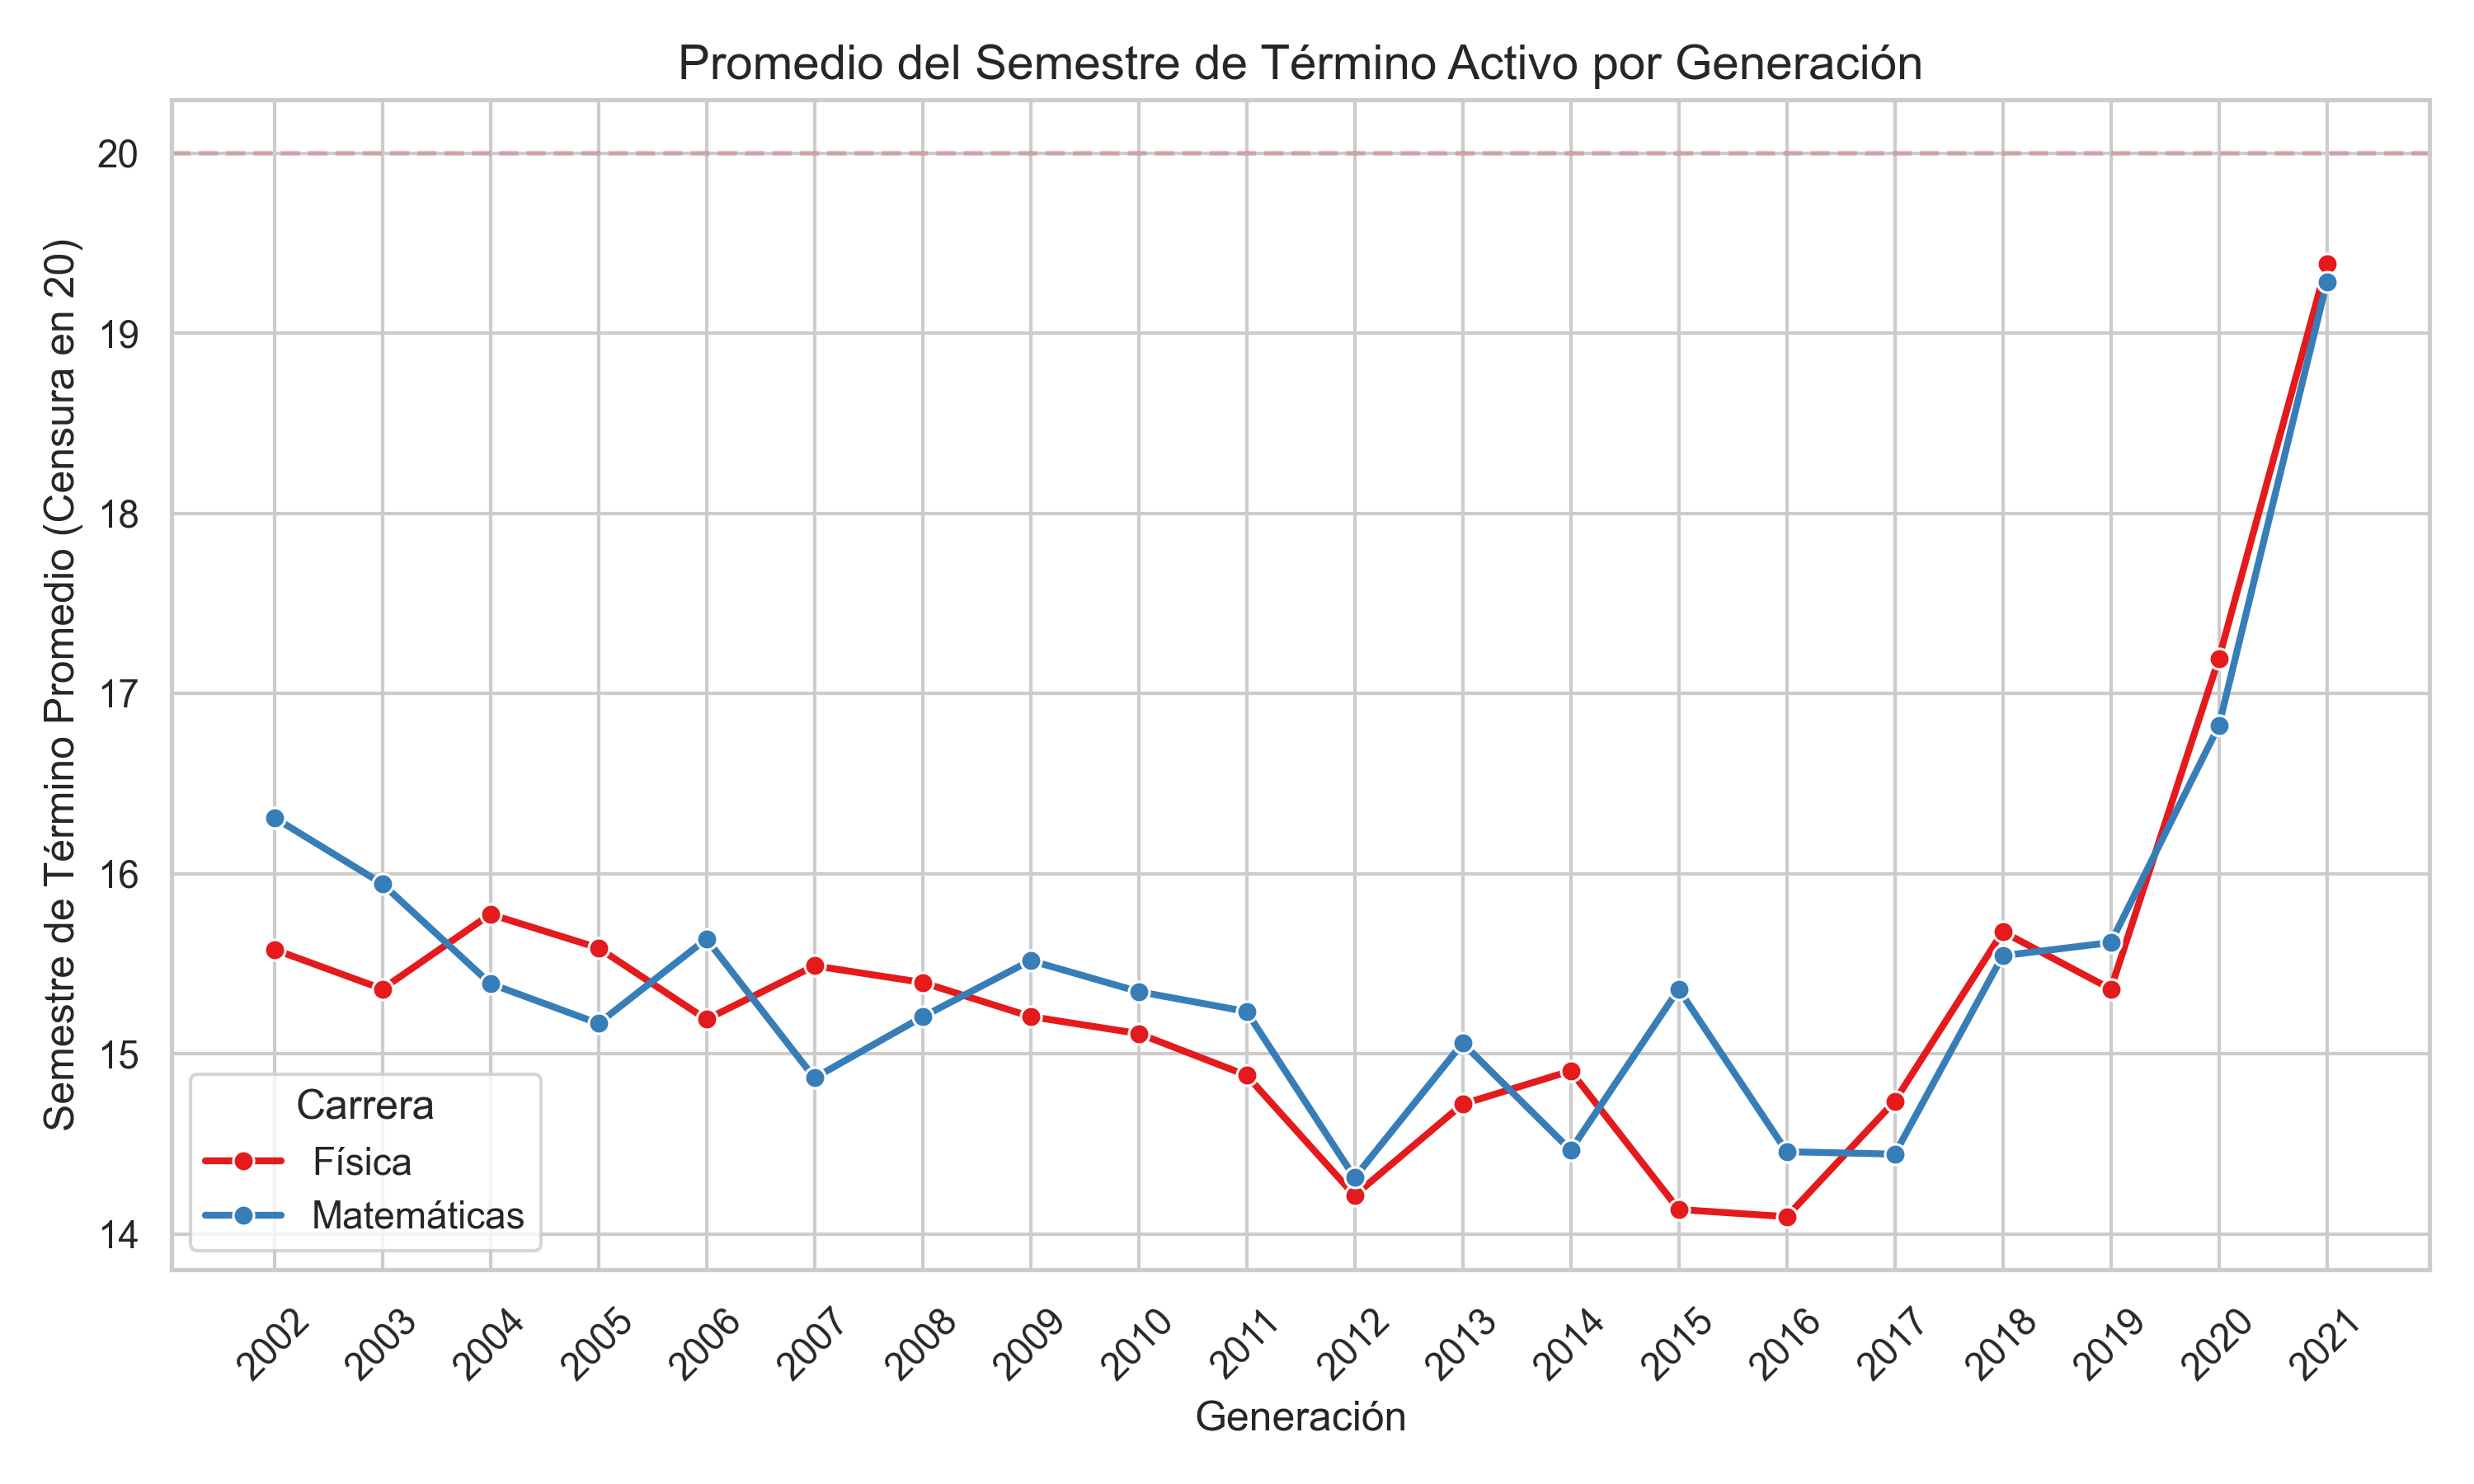
\includegraphics[width=0.8\textwidth]{imagenes/eda_media_semestre_termino.png}
    \caption{Evolución de la media del semestre de término activo por generación (Matemáticas vs. Física).}
    \label{fig:eda_media}
\end{figure}

Sin embargo, es fundamental notar que la crecida abrupta que se observa a partir de la generación 2017 no necesariamente implica un deterioro súbito en el rendimiento académico, sino que responde a un artefacto de la \textbf{censura informativa}. En las cohortes más recientes, los estudiantes que eventualmente tardarán 14, 16 o 18 semestres en titularse aún no han transcurrido ese tiempo en la facultad; por lo tanto, en la base de datos actual son contabilizados preventivamente con el valor máximo de 20 semestres.

Para validar esta hipótesis, se generó una comparativa (Figura \ref{fig:comparativa_censura}) contrastando la media total contra la media calculada únicamente sobre los alumnos que ya han concluido sus créditos. Se observa que, al excluir los datos censurados, la tendencia se mantiene estable o incluso descendente en los años recientes, confirmando que el repunte es una distorsión temporal. Este fenómeno de subestimación del éxito y sobreestimación del rezago en cohortes jóvenes será abordado con mayor profundidad en las secciones dedicadas al análisis de supervivencia.

\begin{figure}[H]
    \centering
    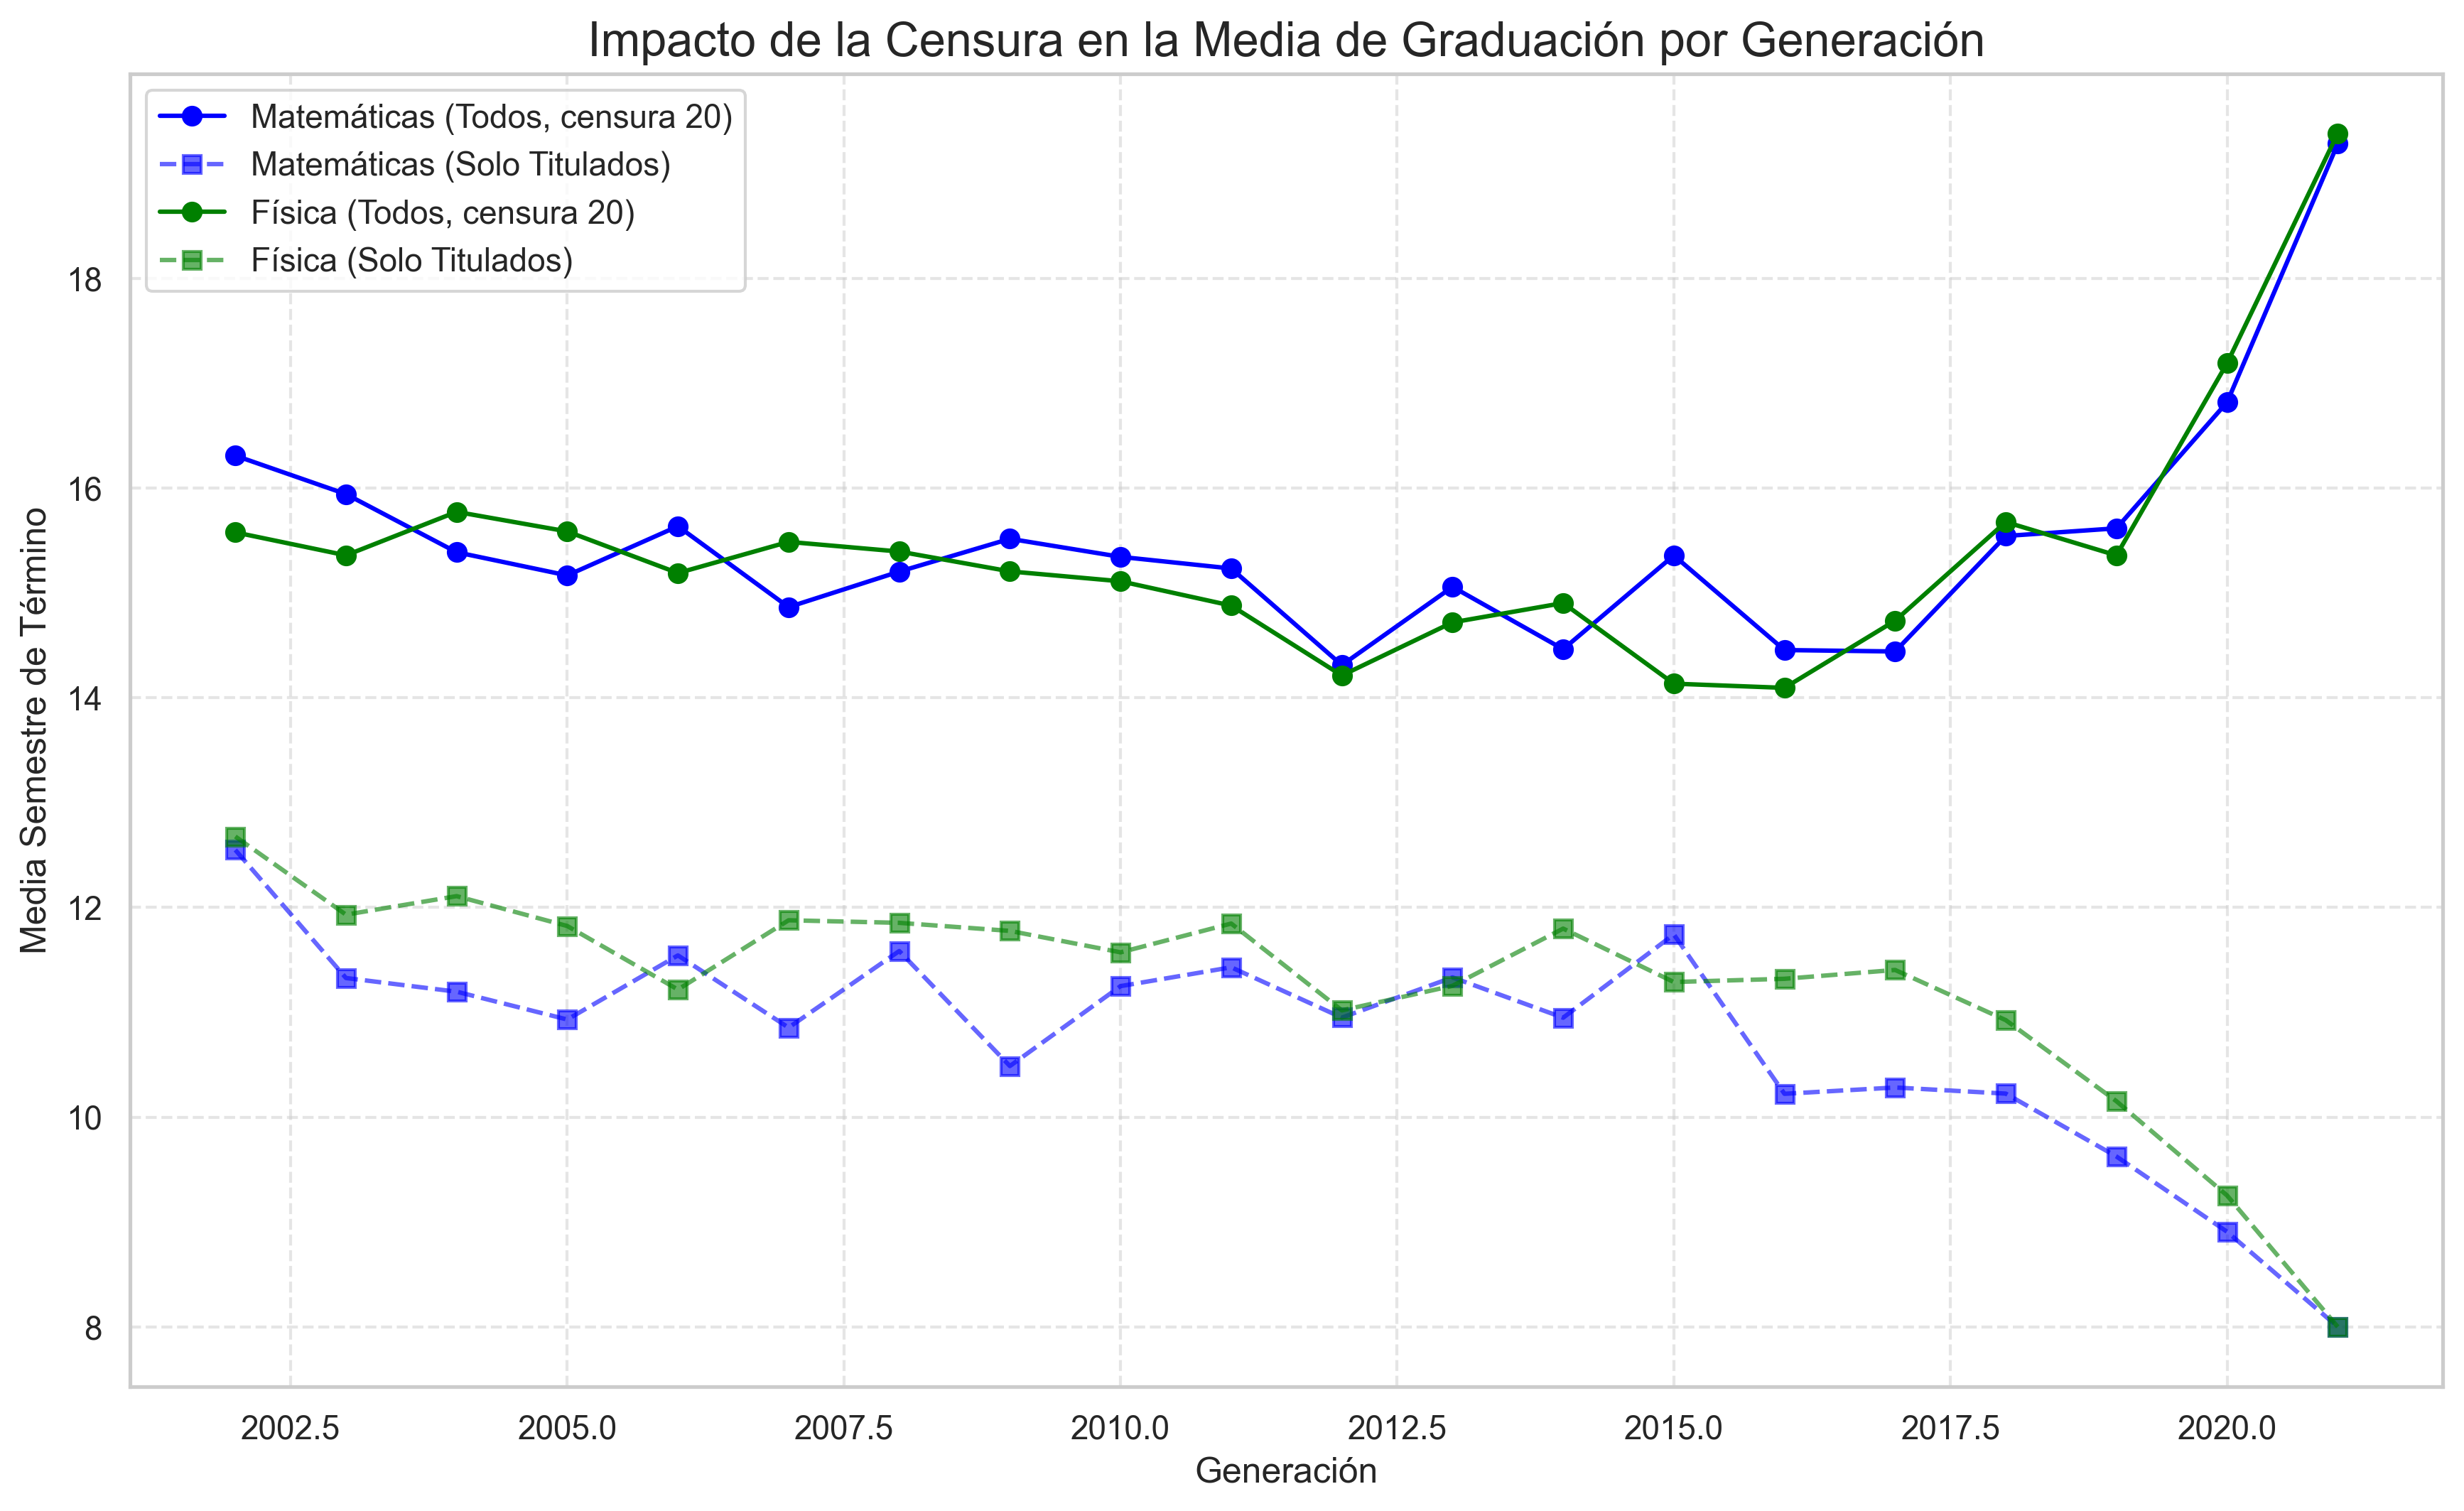
\includegraphics[width=0.8\textwidth]{imagenes/comparativa_censura_media.png}
    \caption{Impacto de la censura en la media generacional: Comparativa entre la muestra total (censurada en $k=20$) y la subpoblación de titulados.}
    \label{fig:comparativa_censura}
\end{figure}

El análisis mediante diagramas de caja (Figura \ref{fig:eda_boxplot}) permite observar que, en las generaciones con trayectorias maduras (2009-2012), el rezago era un evento atípico. Sin embargo, conforme avanzamos hacia 2018, la mediana se desplaza hacia valores superiores a 12 semestres, evidenciando una mayor dispersión en los tiempos de egreso.

\begin{figure}[H]
    \centering
    \begin{minipage}{0.48\textwidth}
        \centering
        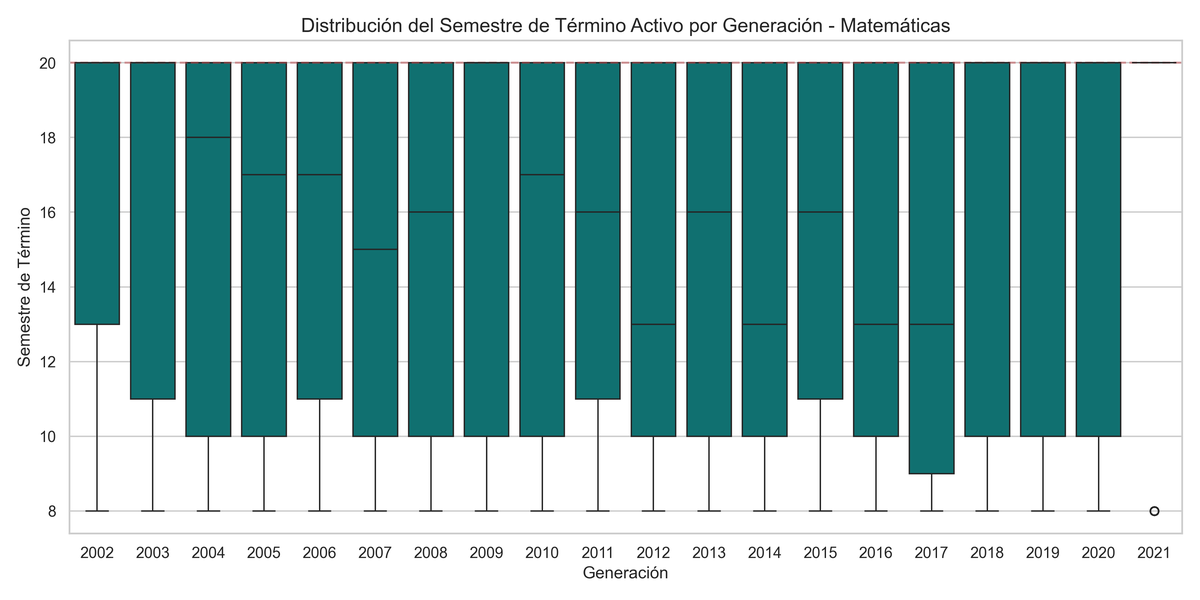
\includegraphics[width=\textwidth]{imagenes/eda_boxplot_gen_matematicas.png}
        \caption{Distribución por generación (Matemáticas).}
    \end{minipage}
    \hfill
    \begin{minipage}{0.48\textwidth}
        \centering
        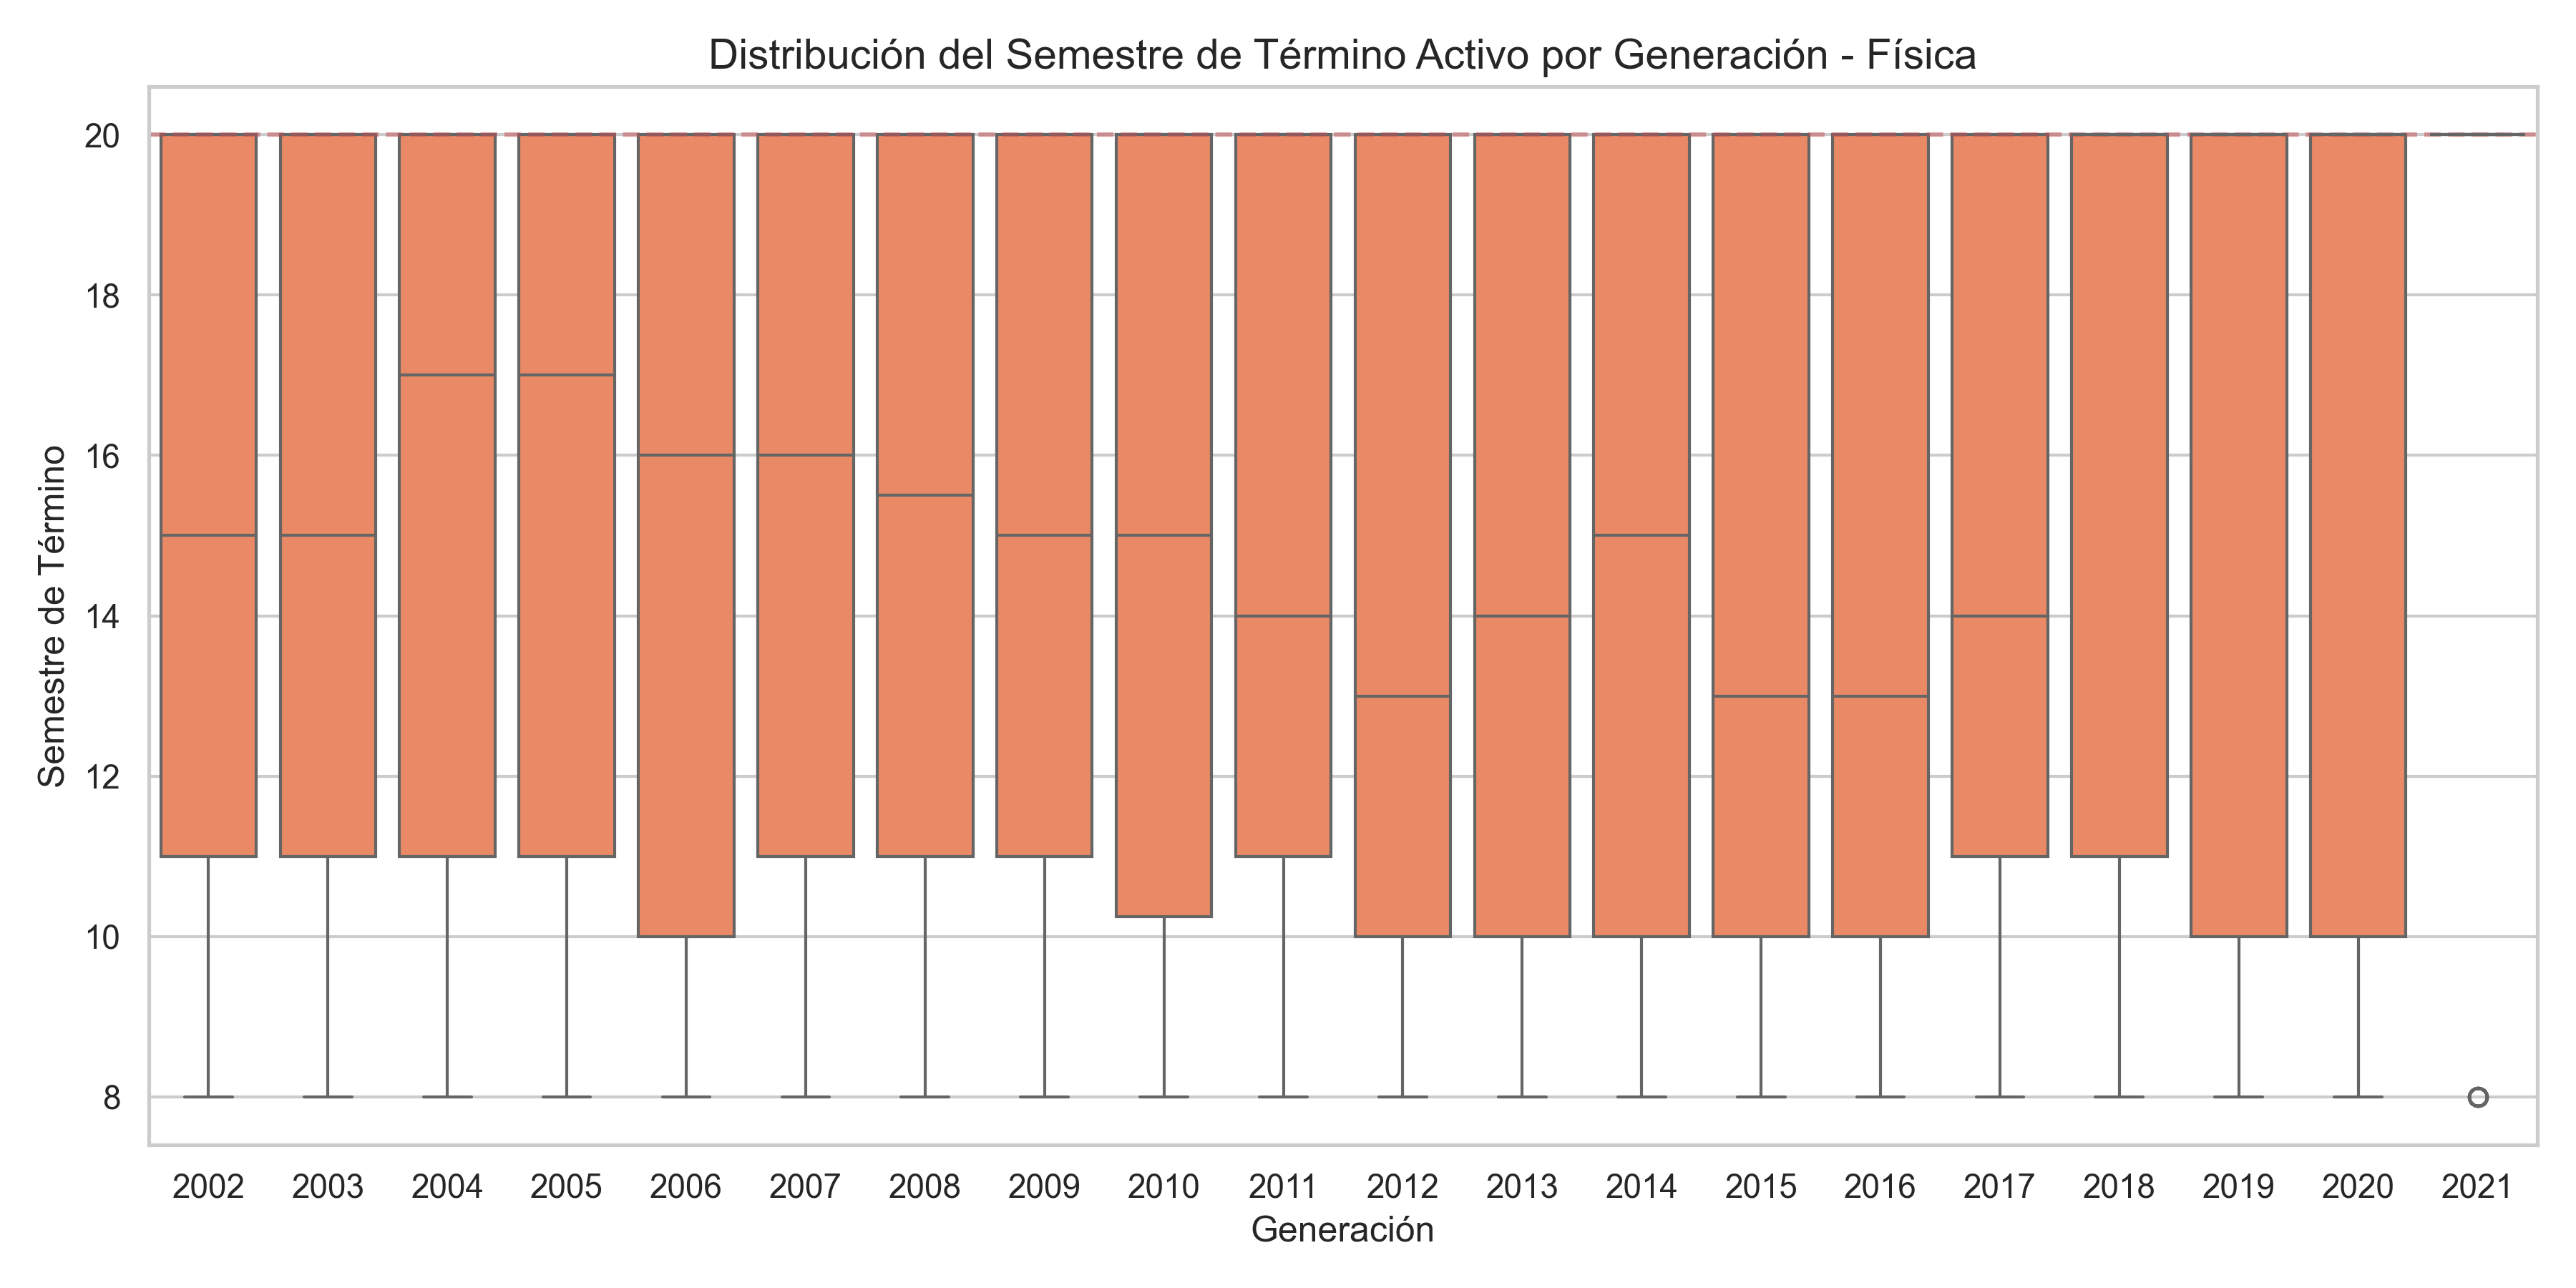
\includegraphics[width=\textwidth]{imagenes/eda_boxplot_gen_fisica.png}
        \caption{Distribución por generación (Física).}
    \end{minipage}
    \label{fig:eda_boxplot}
\end{figure}

\subsection{Divergencia de Trayectorias Académicas}

Para comprender la naturaleza del rezago, es imperativo analizar la evolución temporal de los indicadores de desempeño durante el periodo inicial de formación (S1-S8). Al agrupar a los estudiantes según su tiempo final de egreso ---comparando a quienes no presentan rezago frente a quienes experimentan rezago severo--- se observa un fenómeno de divergencia sistemática y prematura.

Como se ilustra en la Figura \ref{fig:evolucion_metricas}, la separación entre los perfiles académicos no ocurre al final de la trayectoria reglamentaria, sino que comienza a manifestarse desde el segundo y tercer semestre. Los intervalos de confianza al 95\% (áreas sombreadas) confirman que estas diferencias son estadísticamente significativas desde etapas muy tempranas, especialmente en variables críticas como el \textit{Promedio Real} y el \textit{Índice de Esfuerzo}.

\begin{figure}[H]
    \centering
    \begin{minipage}{0.48\textwidth}
        \centering
        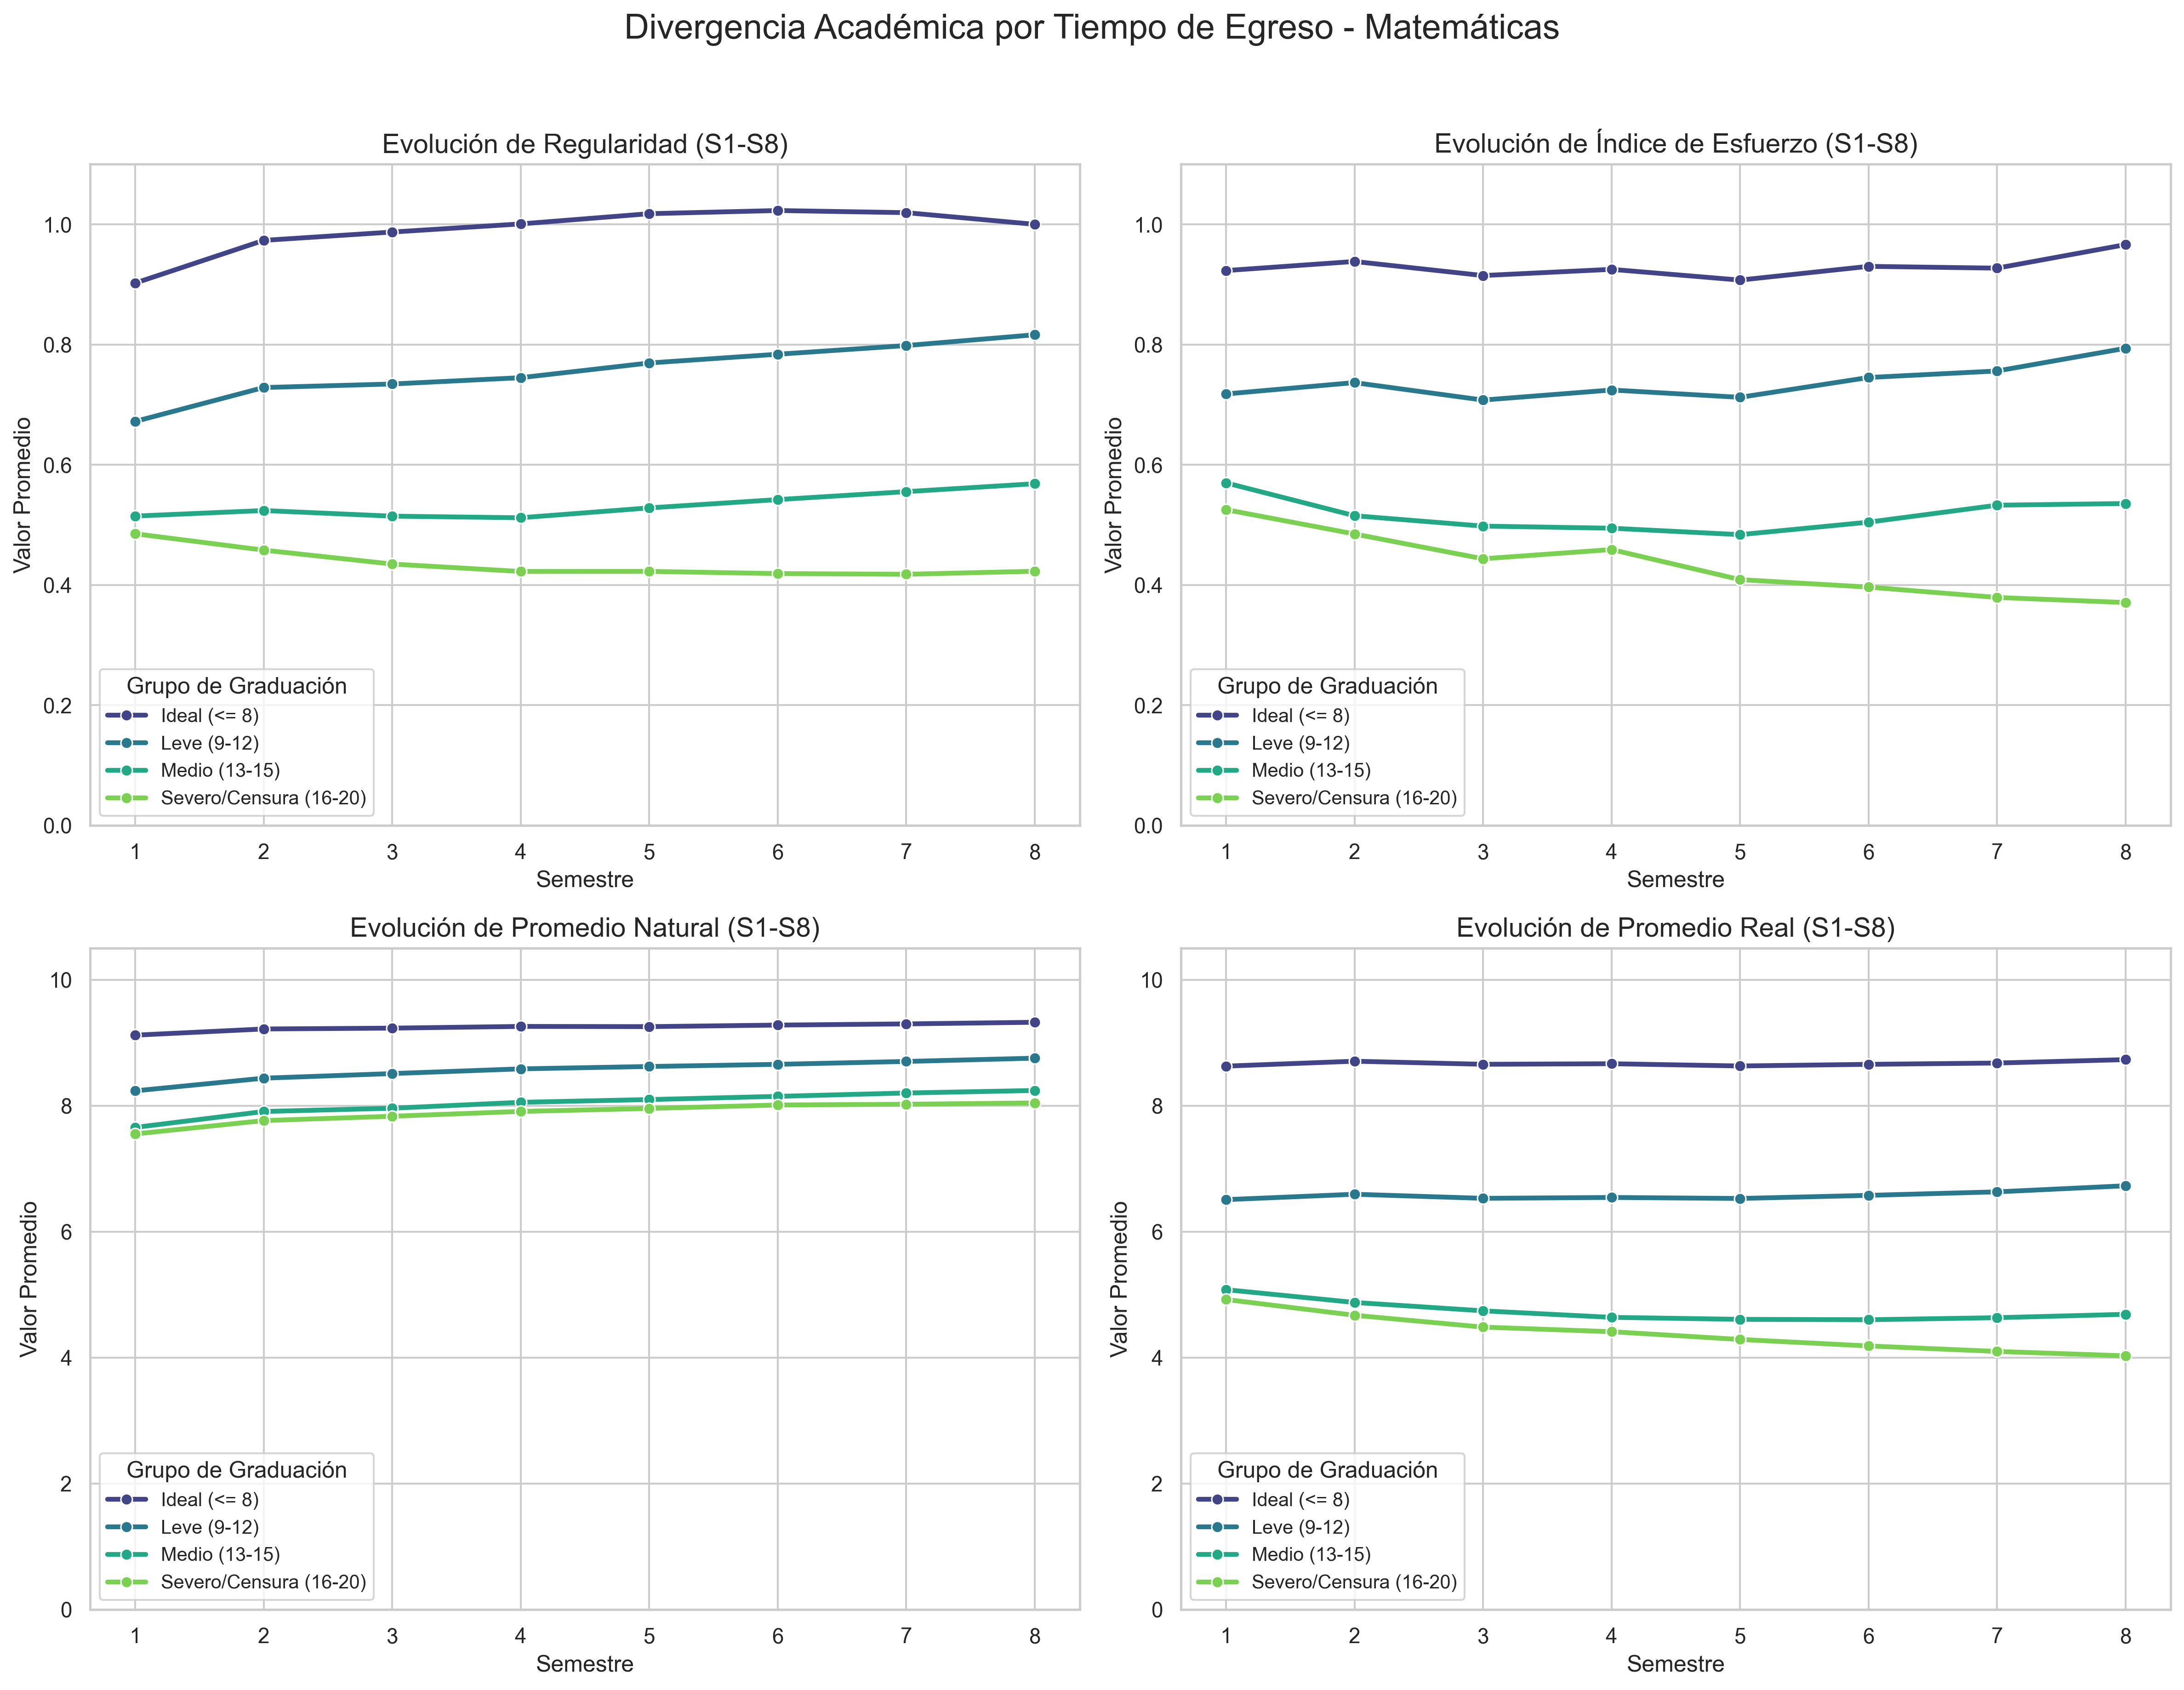
\includegraphics[width=\textwidth]{imagenes/evolucion_metricas_matematicas.png}
        \caption{Evolución de métricas con CI (Matemáticas).}
    \end{minipage}
    \hfill
    \begin{minipage}{0.48\textwidth}
        \centering
        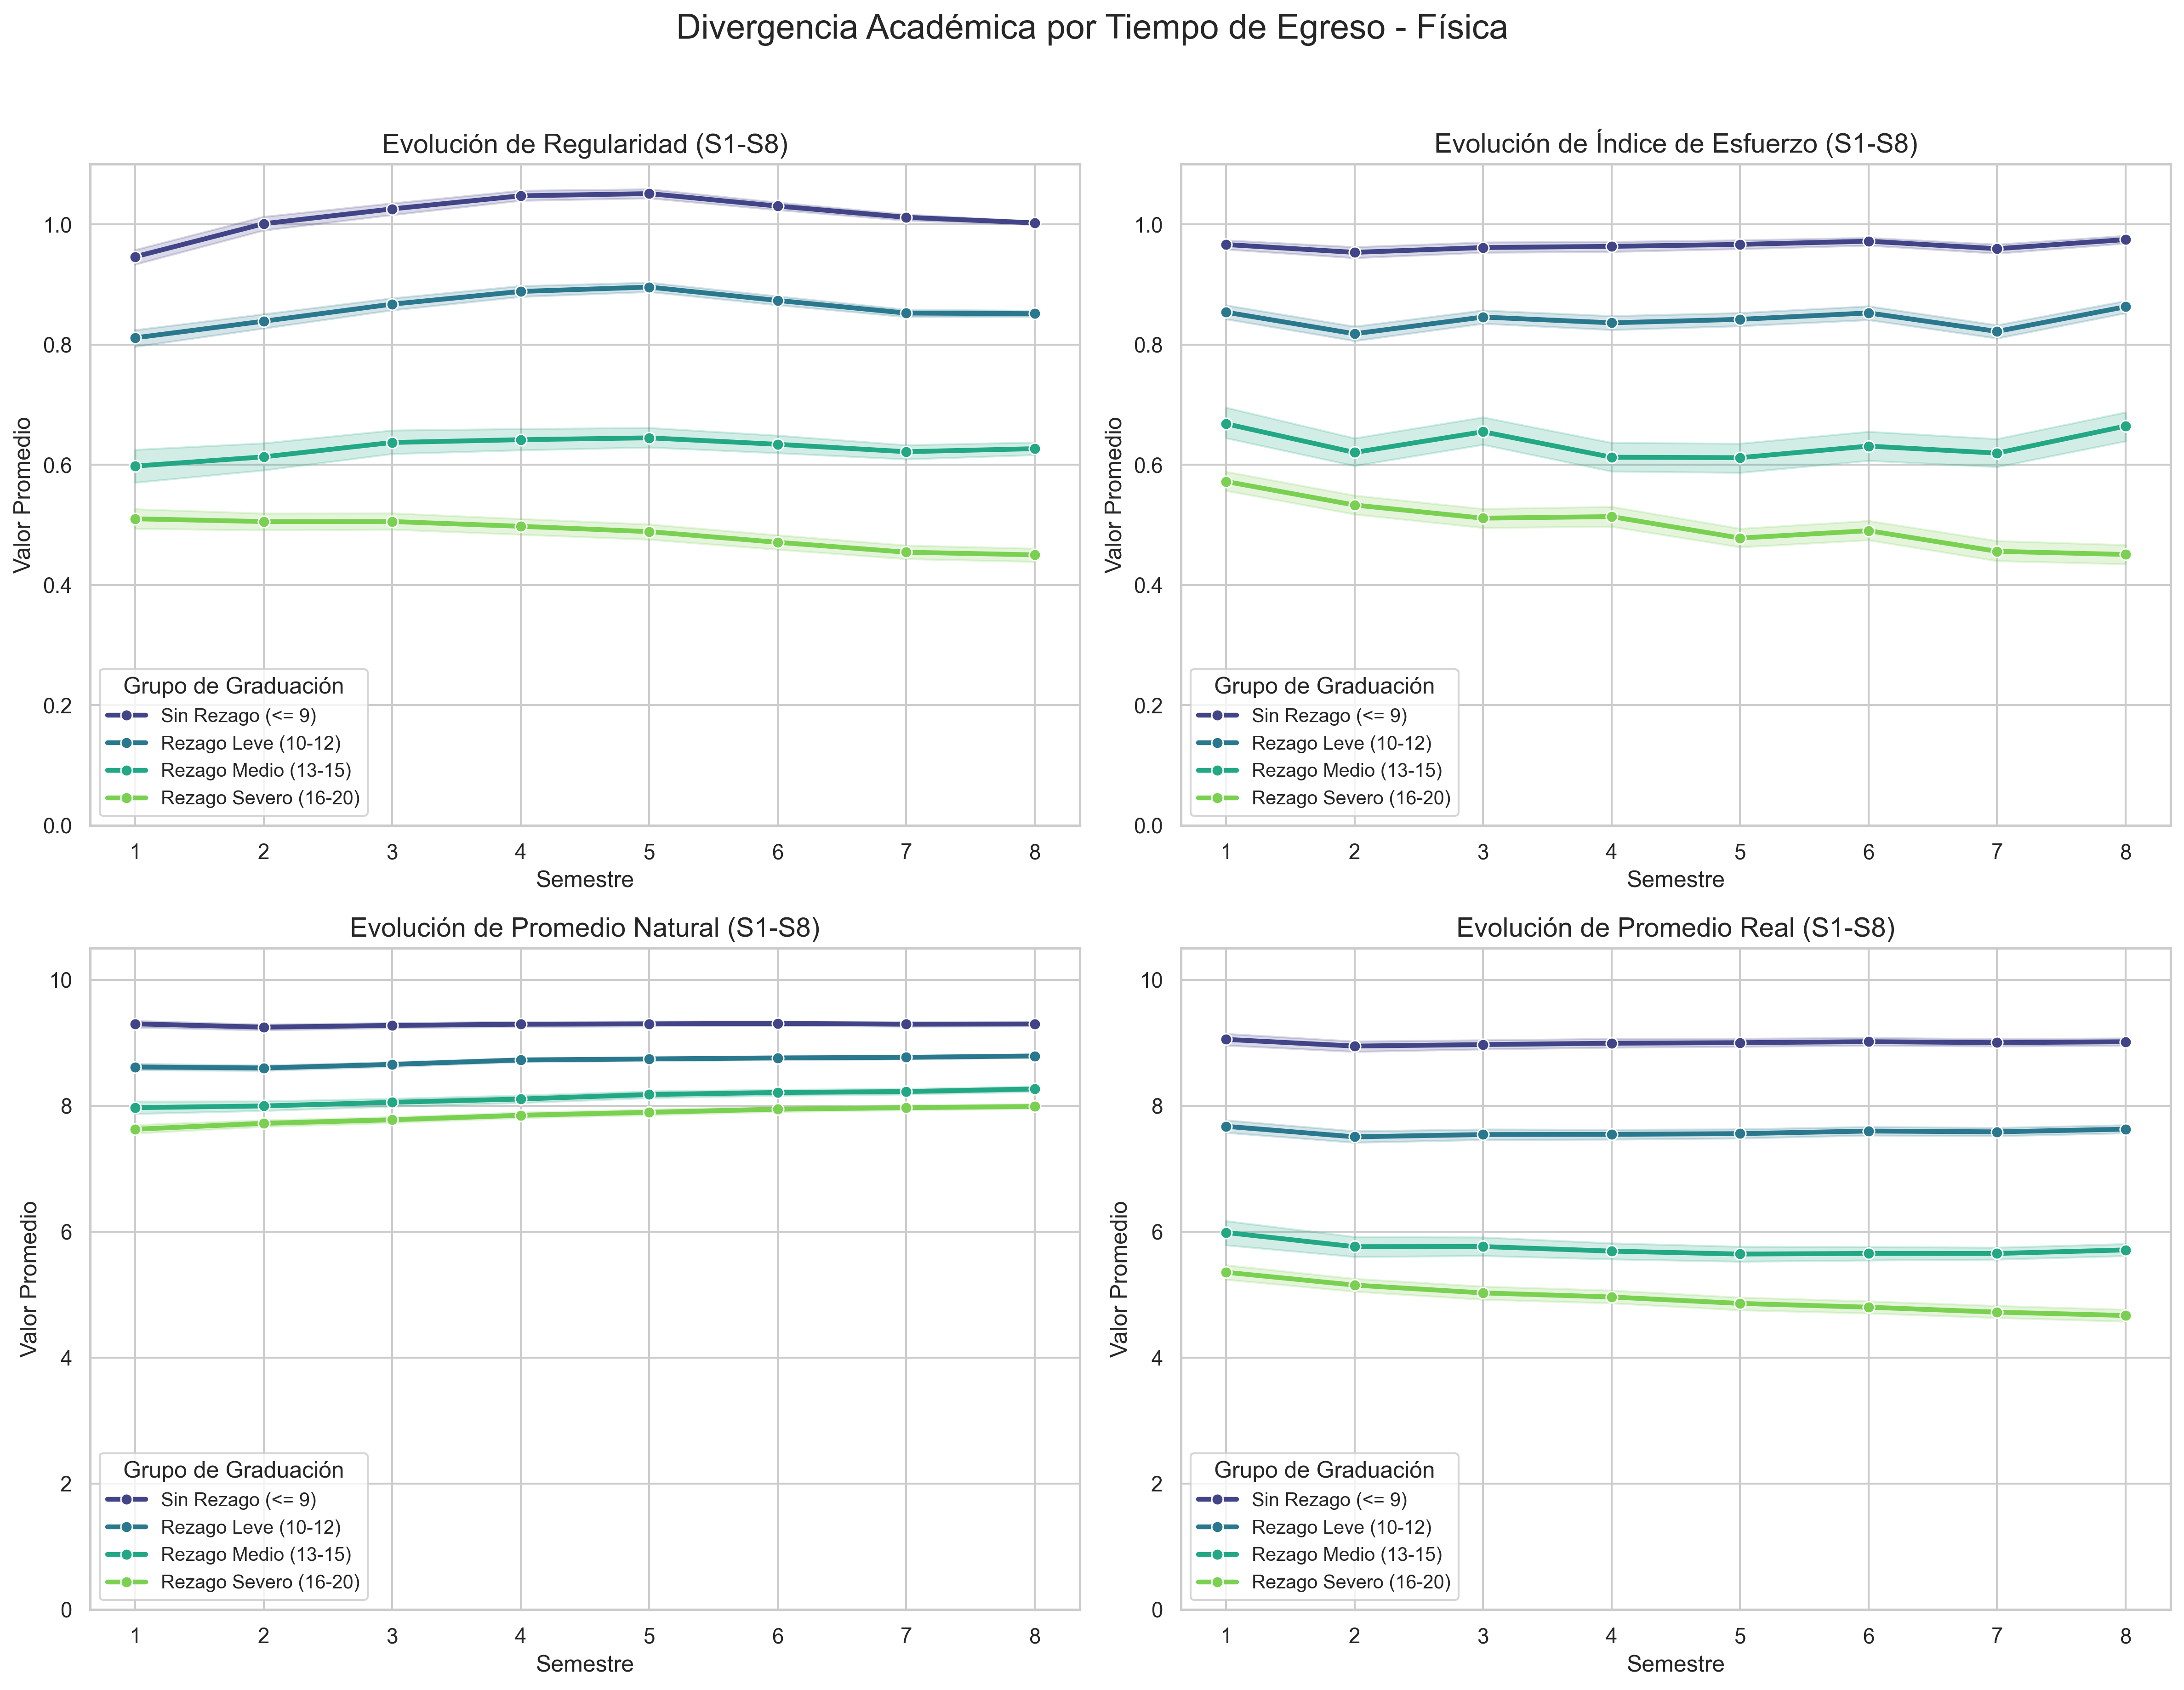
\includegraphics[width=\textwidth]{imagenes/evolucion_metricas_fisica.png}
        \caption{Evolución de métricas con CI (Física).}
    \end{minipage}
    \label{fig:evolucion_metricas}
\end{figure}

Esta evidencia sugiere que el éxito o fracaso académico está fuertemente condicionado por la "inercia" adquirida en los primeros dos años de la carrera, validando la hipótesis de que el rezago es un proceso acumulativo y no un evento aislado del egreso.

\subsection{Análisis de Componentes Principales (PCA)}

Dada la alta dimensionalidad de los predictores (32 variables capturando esfuerzo, promedio y regularidad a lo largo de 8 semestres), se implementó un Análisis de Componentes Principales (PCA) para reducir la complejidad del espacio de estados. El análisis se restringió exclusivamente a los alumnos con trayectorias iniciales completas (S1-S8).

\subsubsection{Varianza Explicada y Estructura de Datos}

Como se detalla en la Tabla \ref{tab:pca_varianza}, el primer componente principal (PC1) captura una proporción masiva de la varianza total (68.9\% en Matemáticas y 75.8\% en Física). Esto sugiere que la trayectoria académica está dominada por un "perfil de rendimiento general" altamente consistente.

\begin{table}[H]
\centering
\begin{tabular}{|l|c|c|c|c|c|}
\hline
\textbf{Componente} & \textbf{PC1} & \textbf{PC2} & \textbf{PC3} & \textbf{PC4} & \textbf{PC5} \\ \hline
Var. Individual (Mat) & 68.9\% & 8.0\% & 6.3\% & 3.1\% & 2.2\% \\ \hline
Var. Acumulada (Mat) & 68.9\% & 76.9\% & 83.2\% & 86.3\% & 88.5\% \\ \hline
Var. Individual (Fís) & 75.8\% & 6.2\% & 4.7\% & 2.4\% & 1.7\% \\ \hline
Var. Acumulada (Fís) & 75.8\% & 82.0\% & 86.8\% & 89.2\% & 90.9\% \\ \hline
\end{tabular}
\caption{Porcentaje de varianza explicada por los primeros cinco componentes principales.}
\label{tab:pca_varianza}
\end{table}

\subsubsection{Interpretación de los Loadings}

Al analizar las cargas (loadings) del PC1, se observa que las variables con mayor peso son los \textbf{Promedios Reales} de los semestres intermedios (S4-S8), como se muestra en la Tabla \ref{tab:pca_loadings}. Esto indica que la "inercia académica" alcanzada a mitad de la carrera es el factor determinante en la configuración de la trayectoria estudiantil.

\begin{figure}[H]
    \centering
    \begin{minipage}{0.48\textwidth}
        \centering
        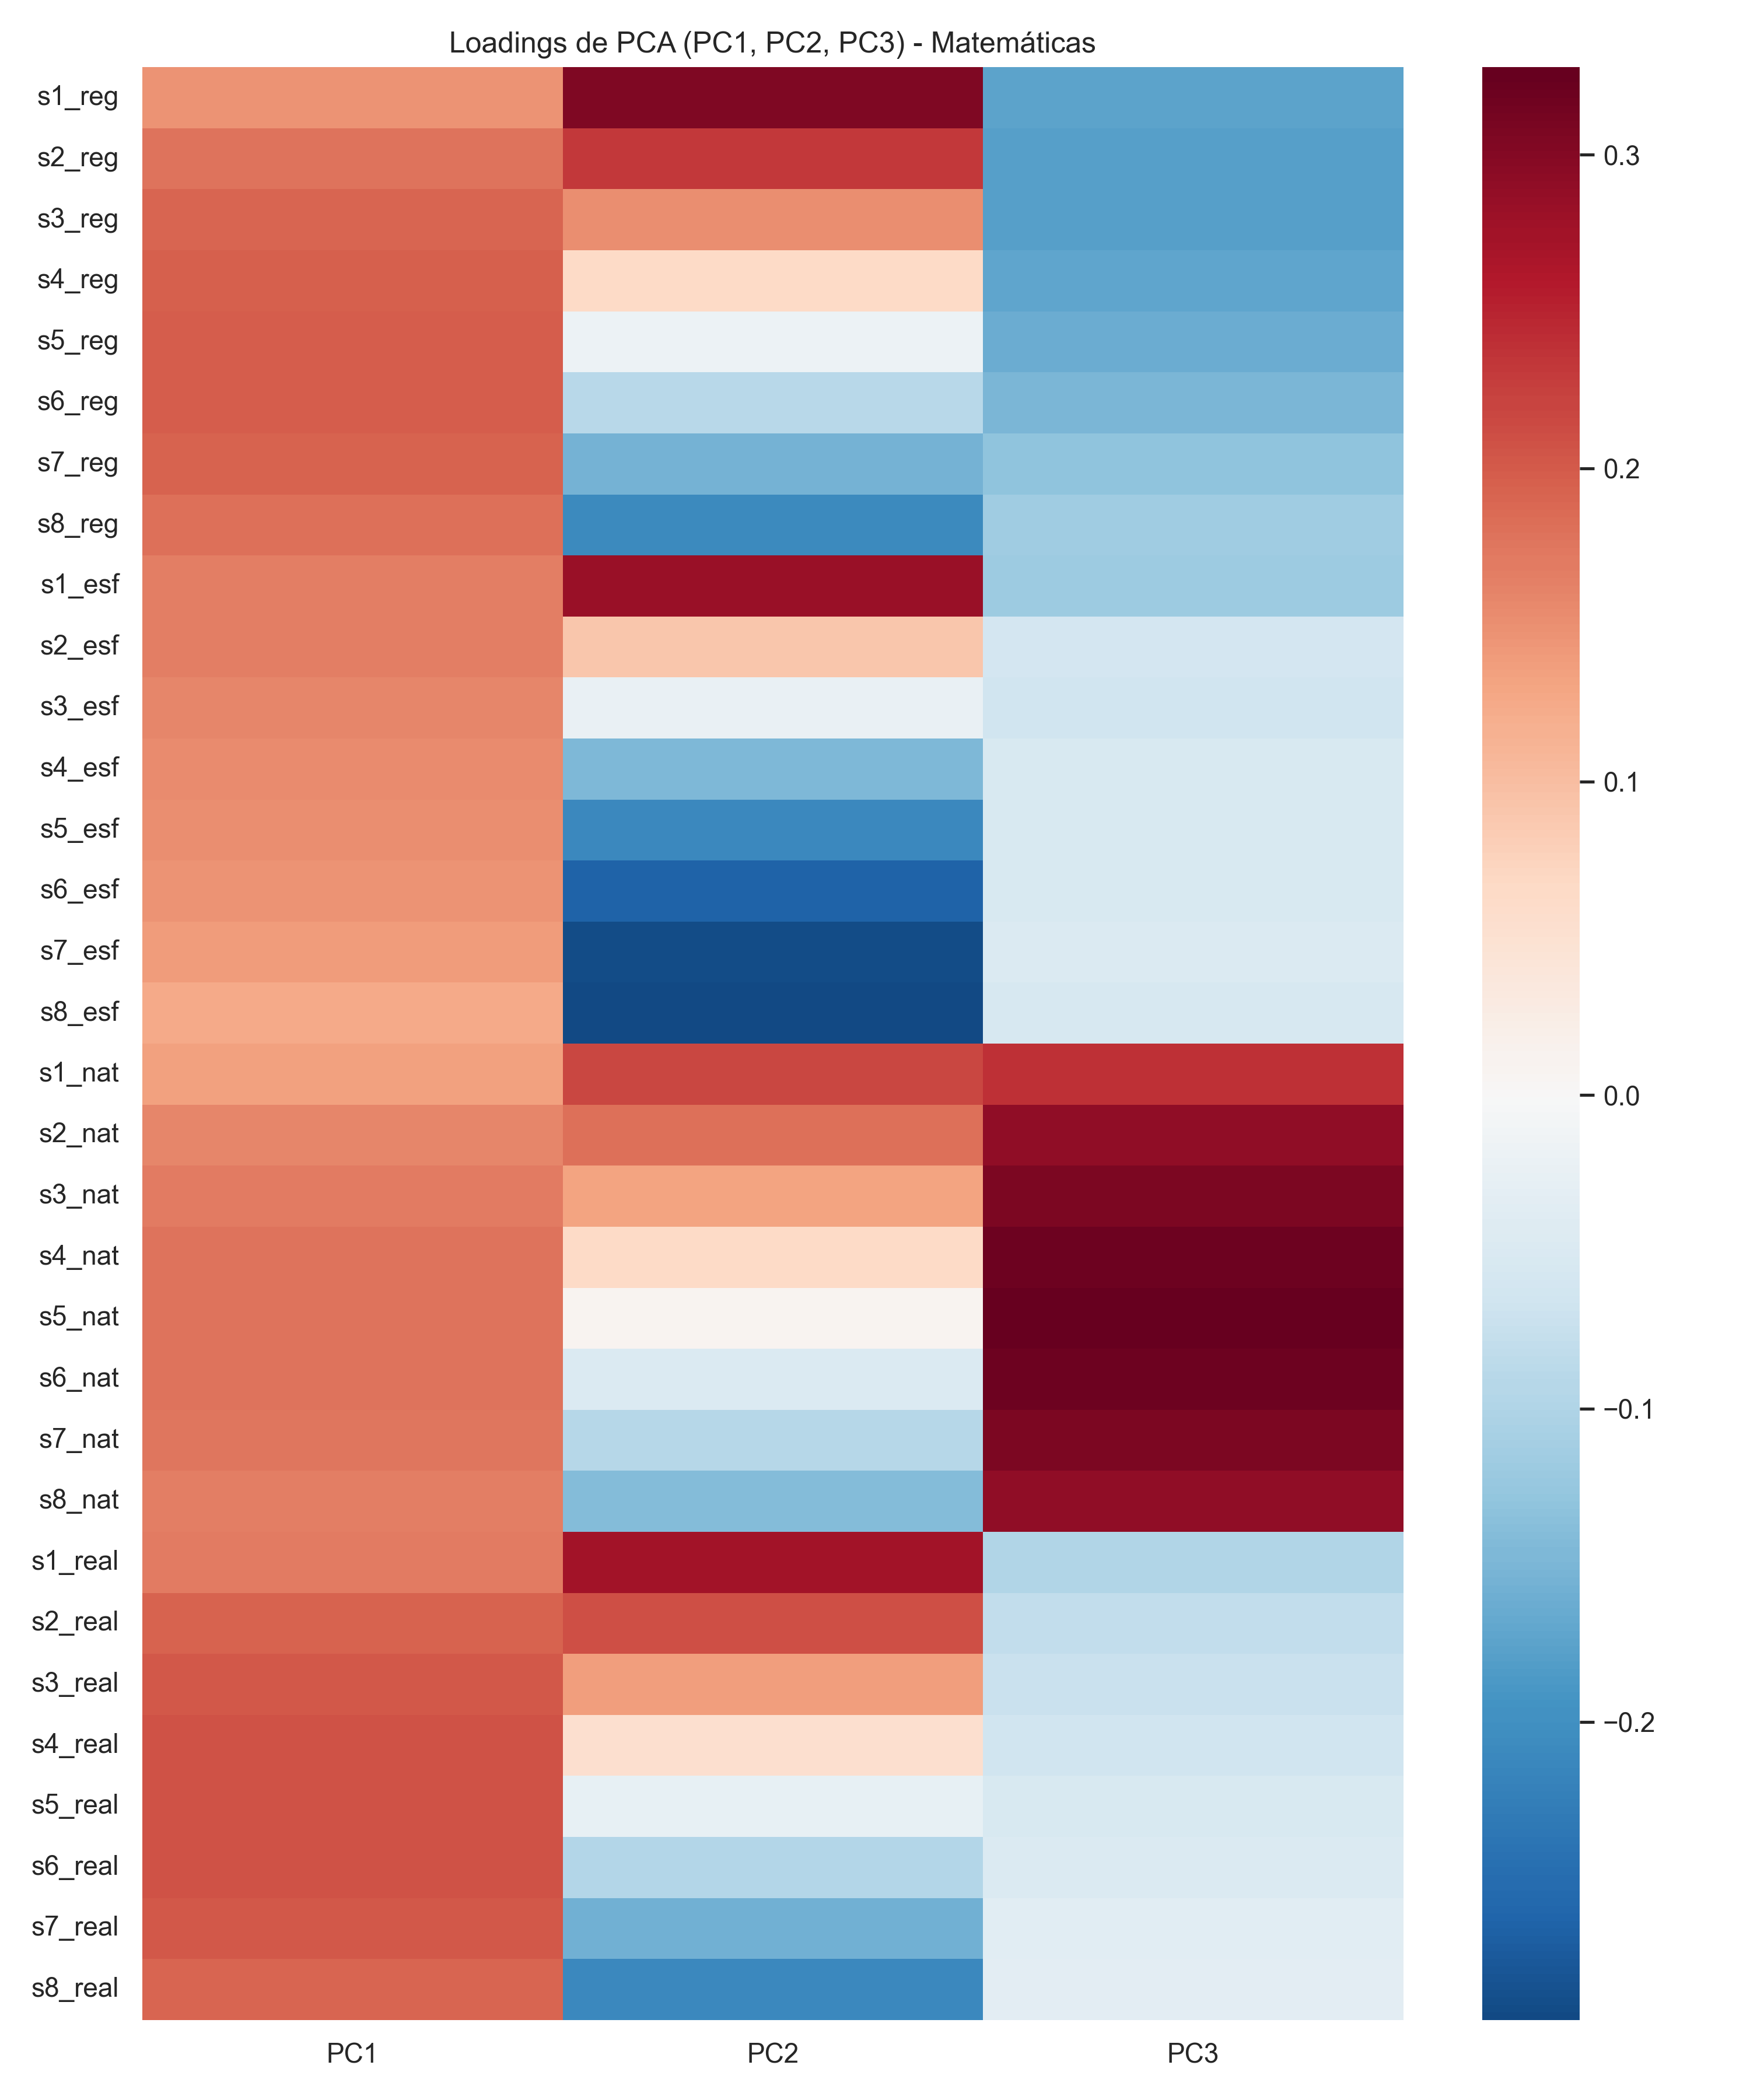
\includegraphics[width=\textwidth]{imagenes/pca_loadings_matematicas.png}
        \caption{Loadings PCA (Matemáticas).}
    \end{minipage}
    \hfill
    \begin{minipage}{0.48\textwidth}
        \centering
        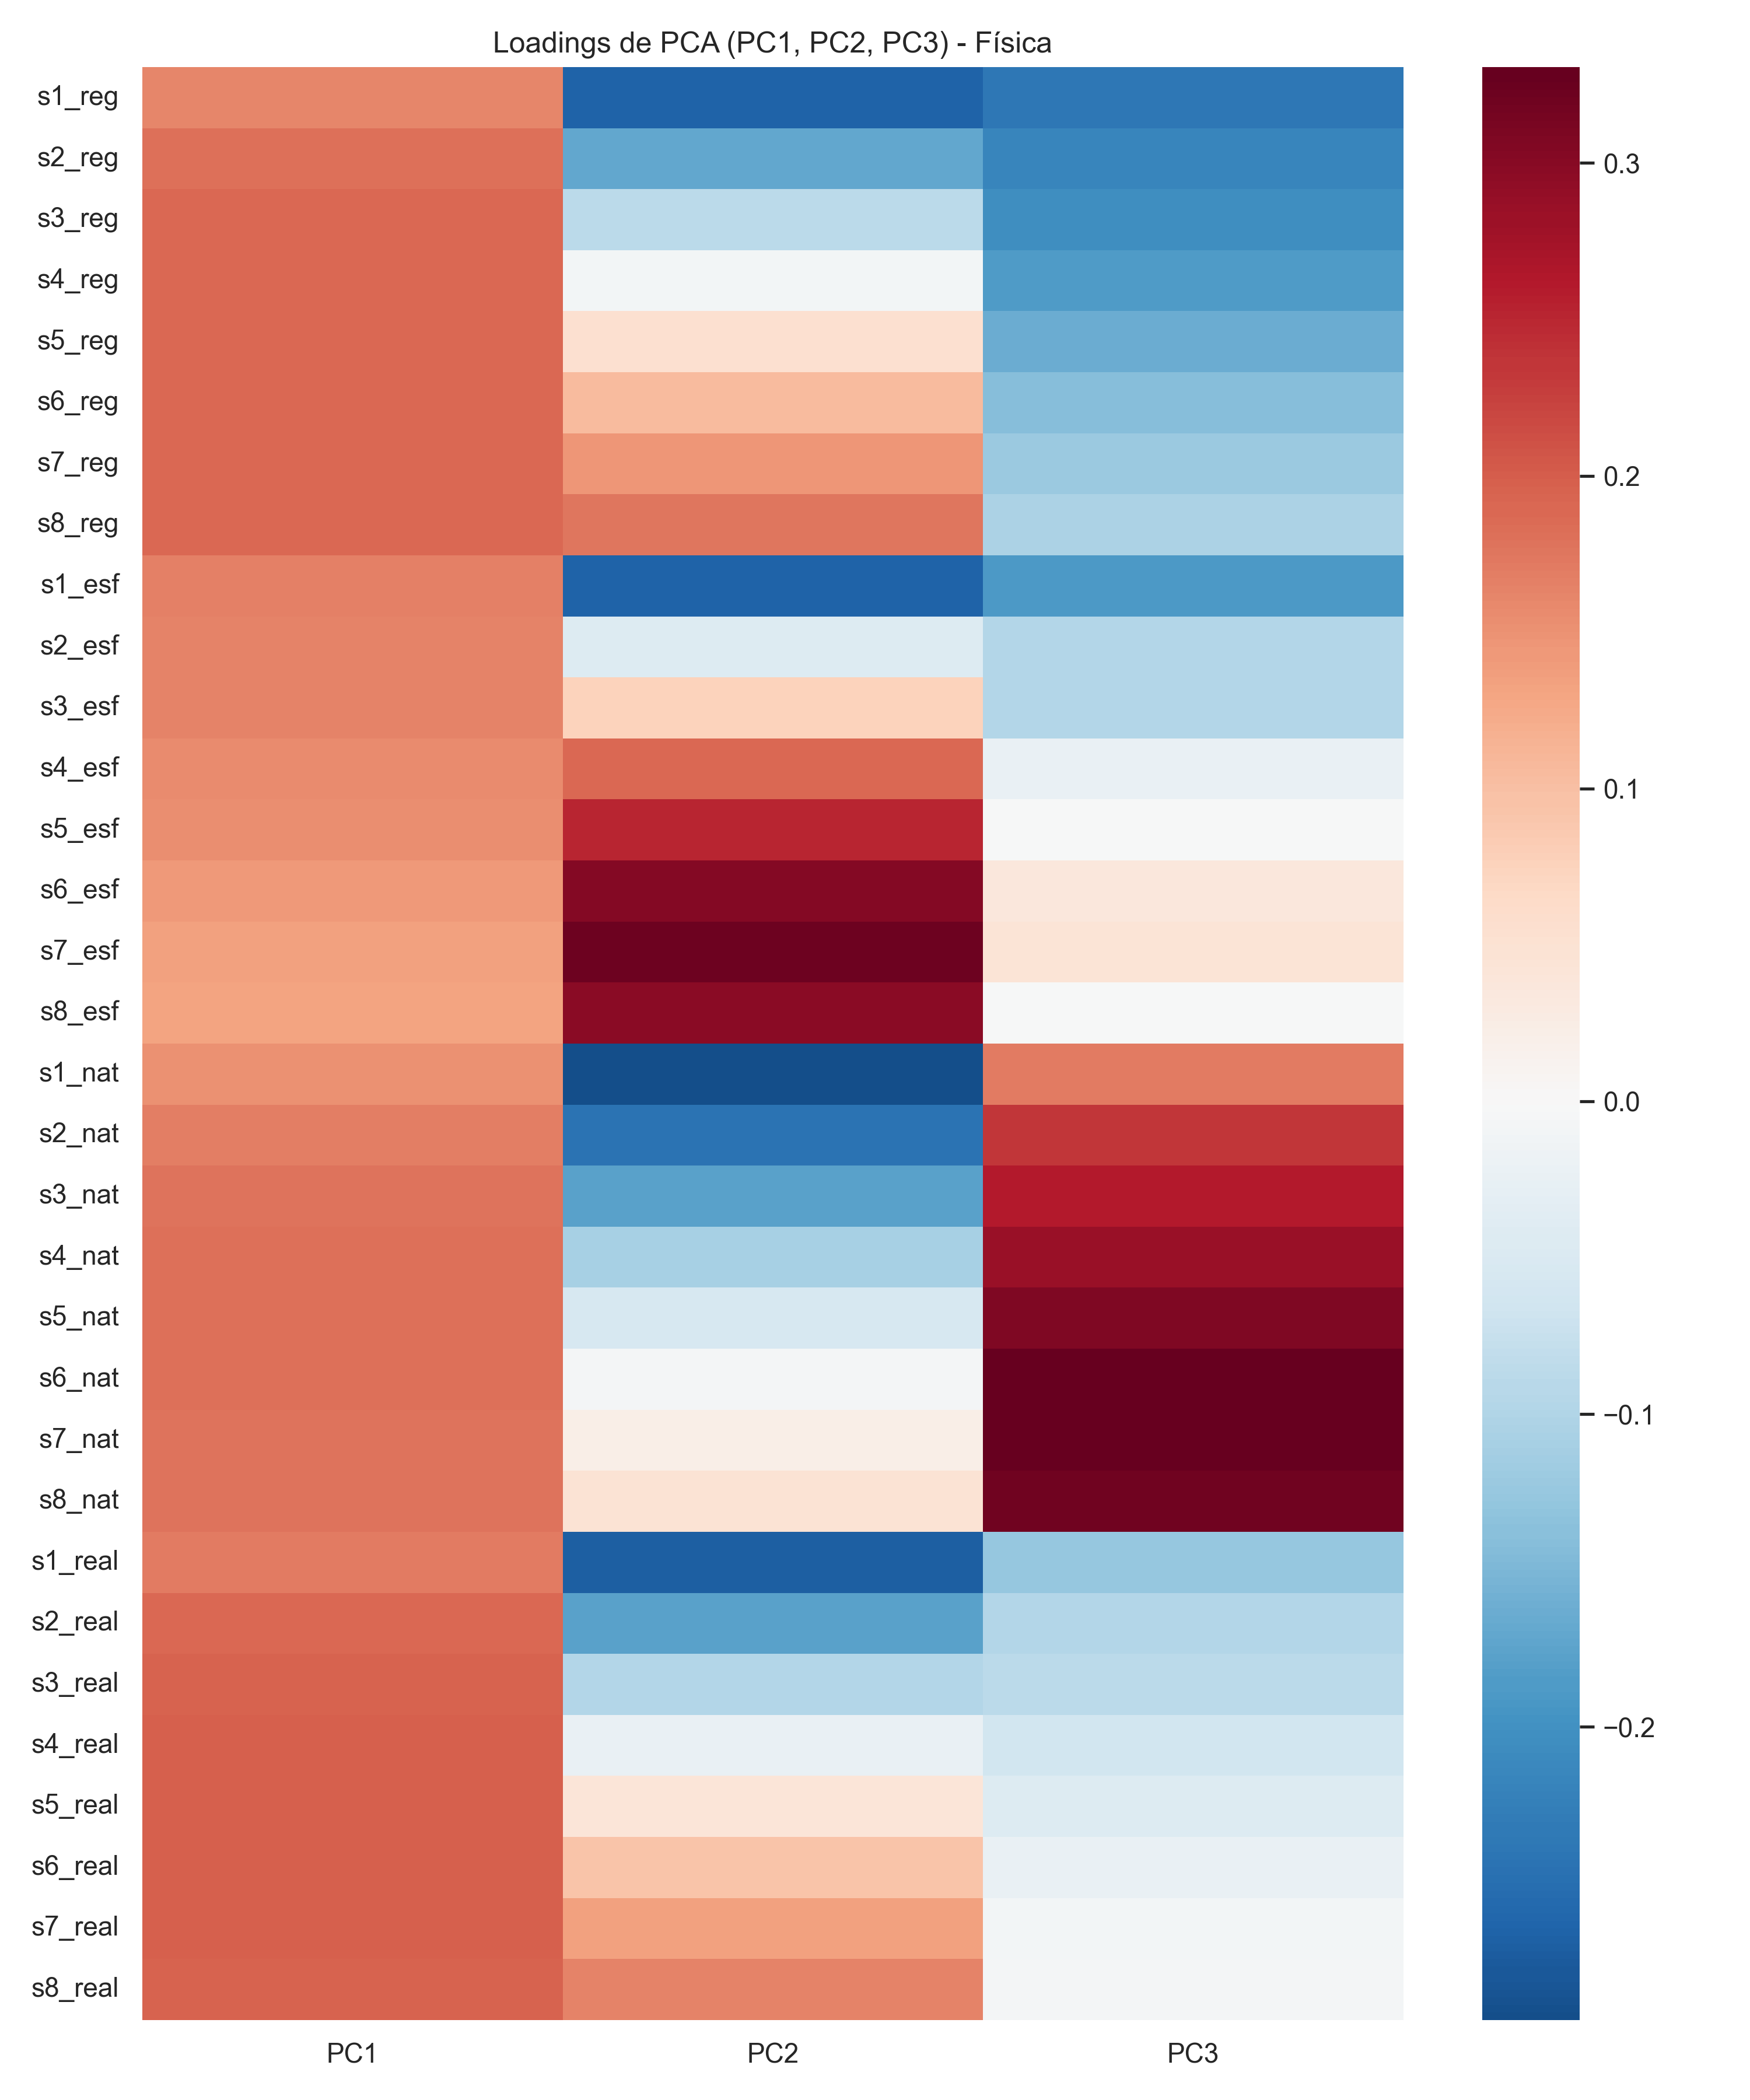
\includegraphics[width=\textwidth]{imagenes/pca_loadings_fisica.png}
        \caption{Loadings PCA (Física).}
    \end{minipage}
    \label{fig:pca_loadings}
\end{figure}

\begin{table}[H]
\centering
\begin{tabular}{|l|l|c|l|l|c|}
\hline
\multicolumn{3}{|c|}{\textbf{Matemáticas}} & \multicolumn{3}{c|}{\textbf{Física}} \\ \hline
\textbf{Rango} & \textbf{Variable} & \textbf{PC1} & \textbf{Rango} & \textbf{Variable} & \textbf{PC1} \\ \hline
1 & s5\_real & 0.205 & 1 & s5\_real & 0.198 \\ \hline
2 & s6\_real & 0.205 & 2 & s6\_real & 0.198 \\ \hline
3 & s4\_real & 0.204 & 3 & s4\_real & 0.197 \\ \hline
4 & s7\_real & 0.203 & 4 & s7\_real & 0.197 \\ \hline
5 & s8\_real & 0.201 & 5 & s8\_real & 0.195 \\ \hline
\end{tabular}
\caption{Principales variables que contribuyen al primer componente principal (PC1).}
\label{tab:pca_loadings}
\end{table}

\subsubsection{Visualización del Espacio Latente}

La proyección de los estudiantes en el espacio definido por PC1 y PC2 (Figura \ref{fig:pca_scatter}) revela una gradación continua y nítida respecto a la variable objetivo (\texttt{semestre\_termino}). Los alumnos que egresan en periodos cortos se agrupan en un extremo del eje latente, mientras que aquellos con rezago se desplazan sistemáticamente hacia el polo opuesto. Esta separación natural valida el uso de los componentes principales como predictores robustos para modelos de aprendizaje automático posteriores.

\begin{figure}[H]
    \centering
    \begin{minipage}{0.48\textwidth}
        \centering
        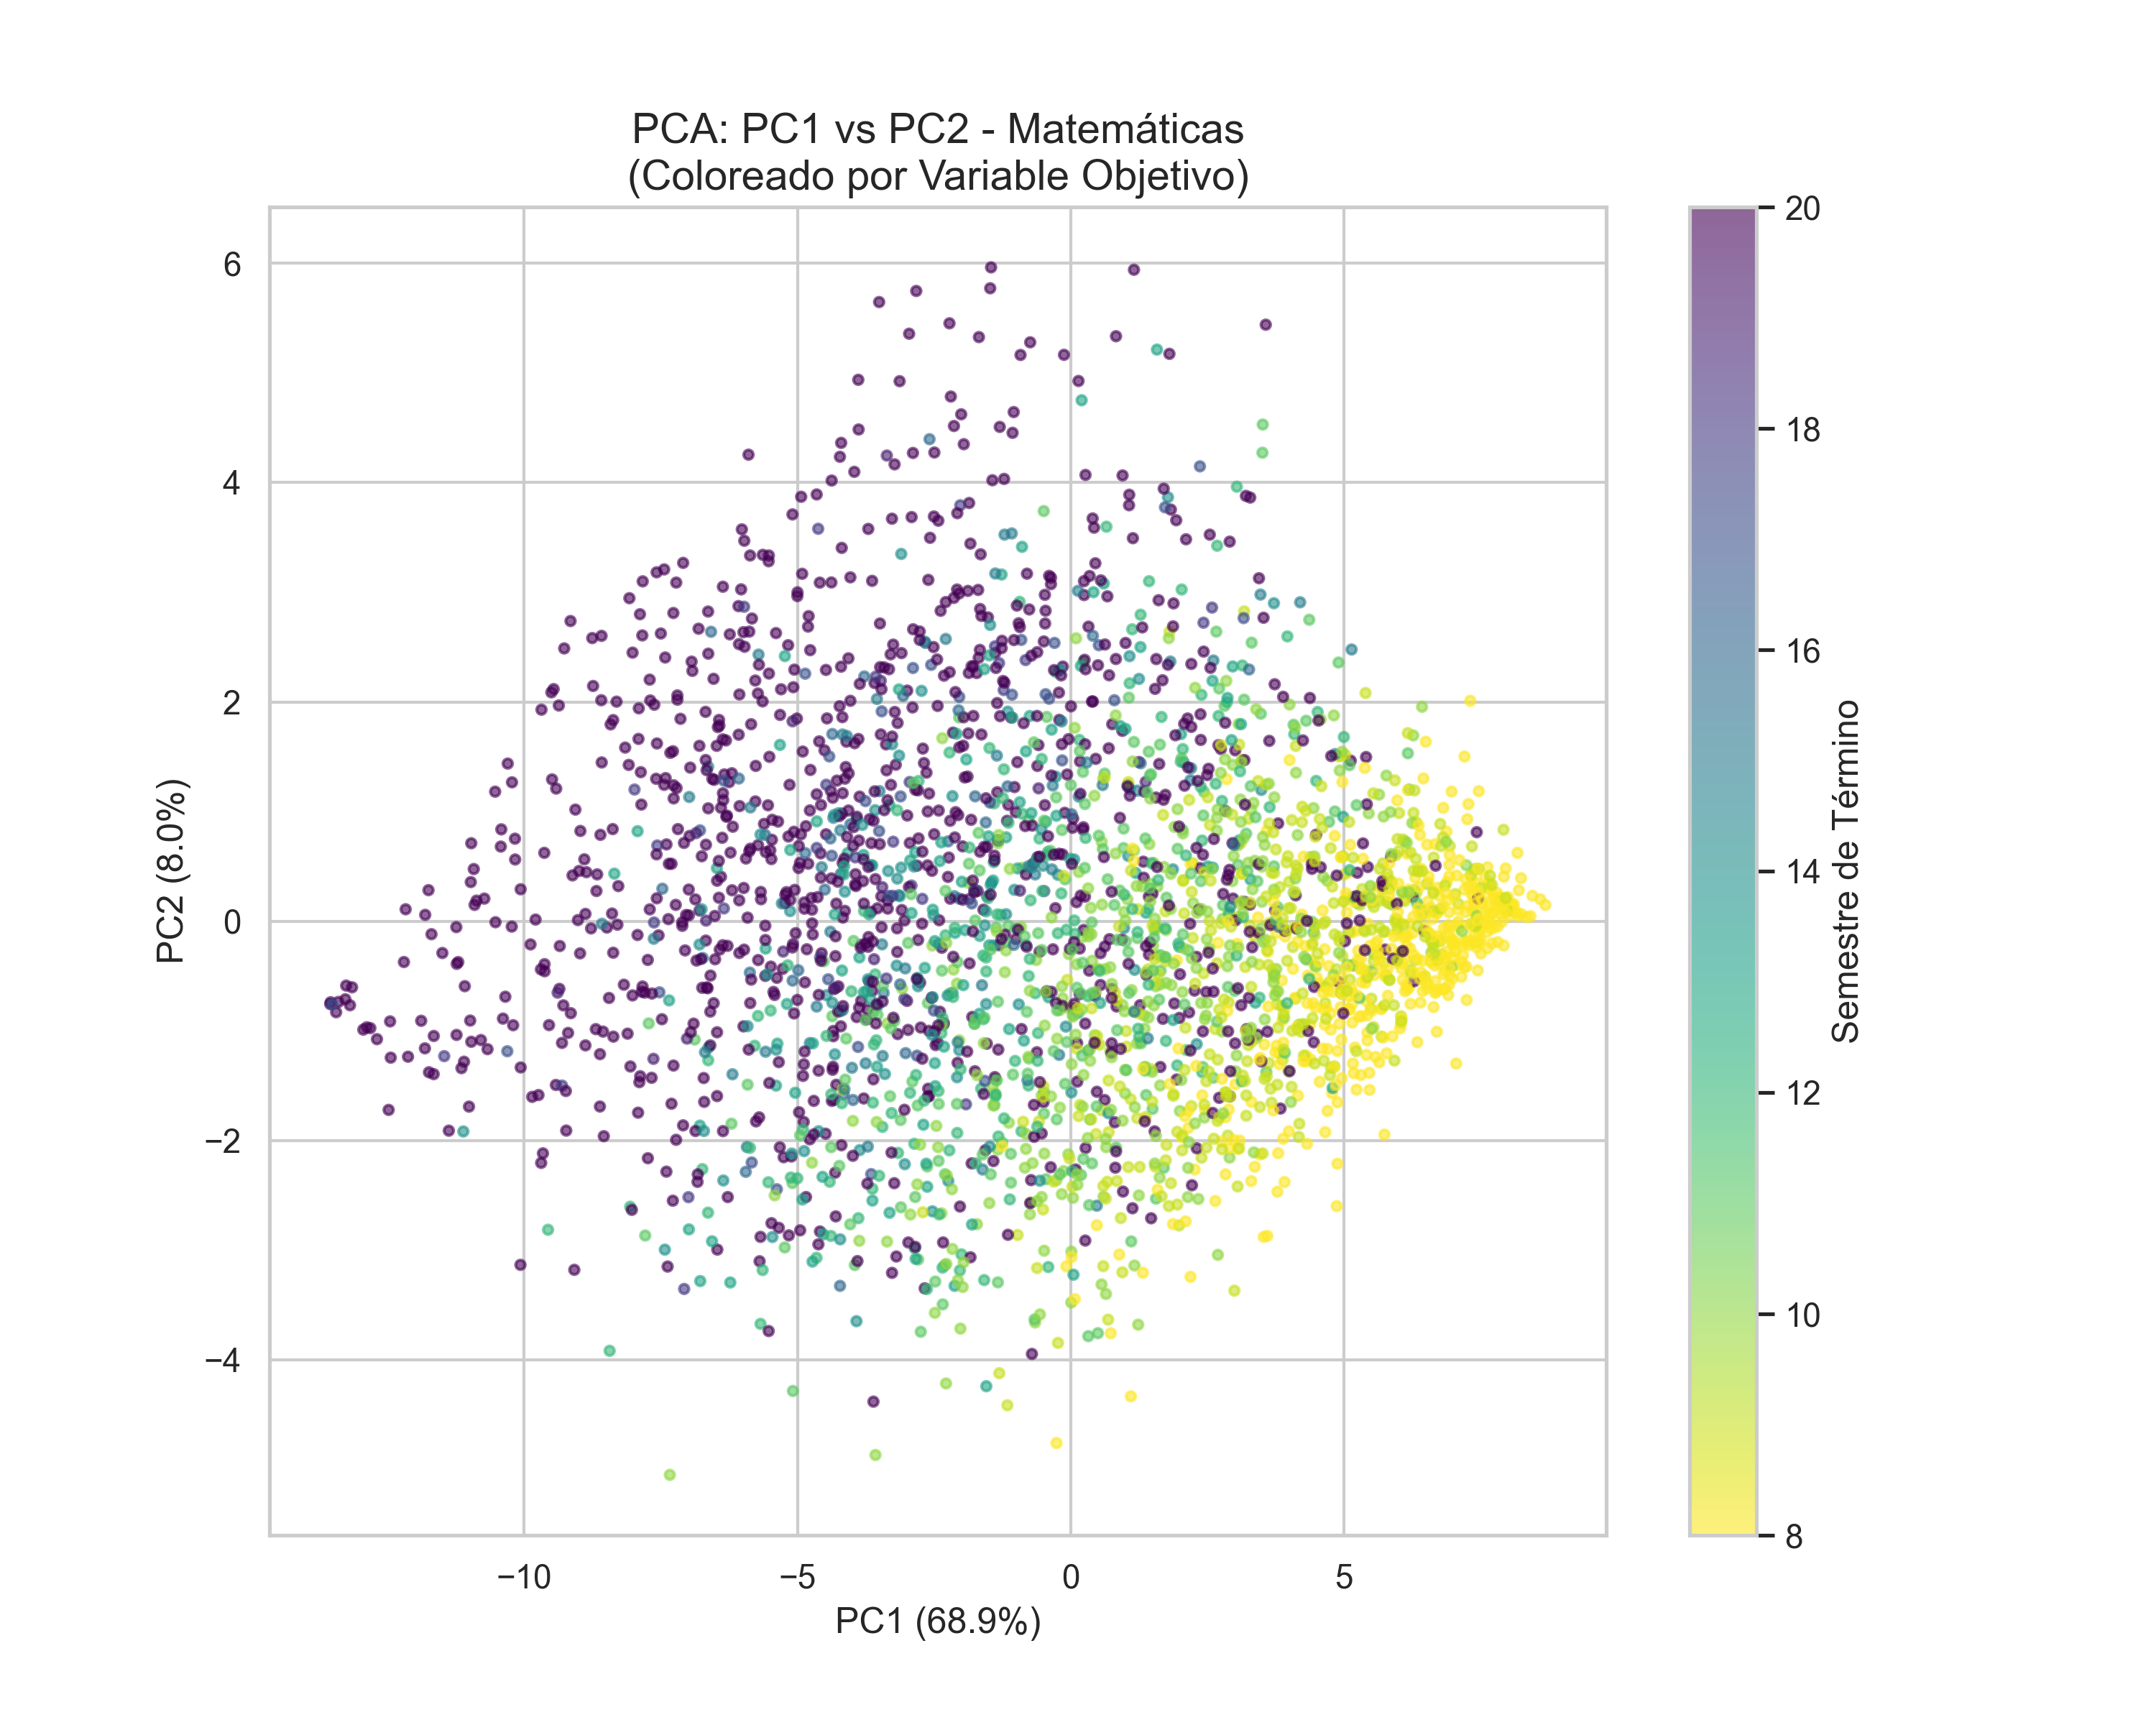
\includegraphics[width=\textwidth]{imagenes/pca_scatter_matematicas.png}
        \caption{Proyección latente (Matemáticas).}
    \end{minipage}
    \hfill
    \begin{minipage}{0.48\textwidth}
        \centering
        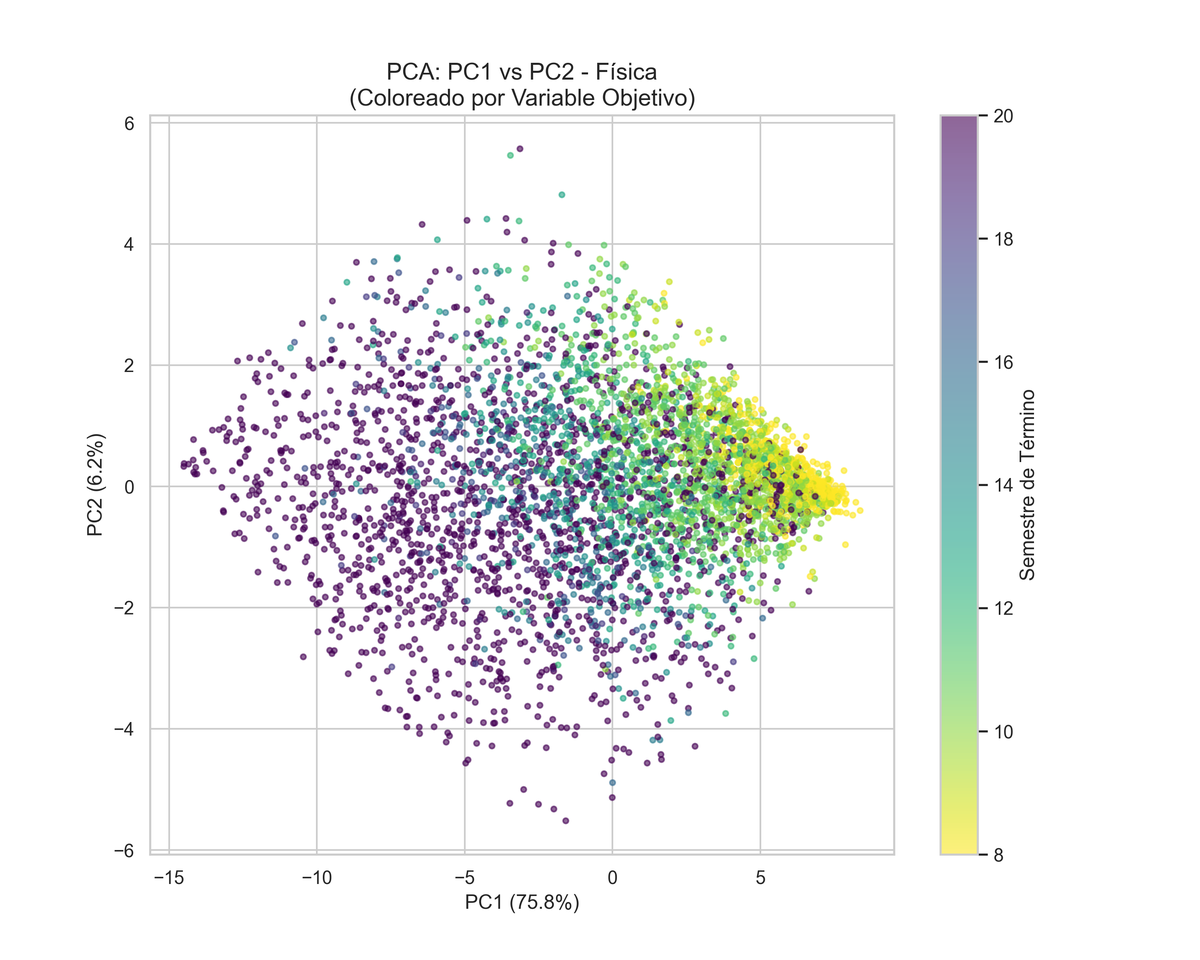
\includegraphics[width=\textwidth]{imagenes/pca_scatter_fisica.png}
        \caption{Proyección latente (Física).}
    \end{minipage}
    \label{fig:pca_scatter}
\end{figure}
